\chapter{Introduction}

    Dans ce dernier livrable, nous allons parler de la conception détaillée de l'application. On expliquera essentiellement la partie serveur de celle-ci puisque la partie client ne se compose que d'une interface qui sera traitée dans le rapport destiné au module d'IHM. De même, nous n'avons pas de base de données, notre application étant accessible en ligne, il aurait été inutile de dupliquer le serveur GTD.\\
    On rappelle que notre application Web utilise GWT pour l'interface et assure la synchronisation entre deux serveurs GTD : celui développé dans le cadre de ce projet multi-modules et le serveur propriétaire Toodledo.

\section{Organisation du chapitre}

    Dans un premier temps, on parlera brièvement de l'architecture physique de l'application. Puis dans un second, on justifiera les différentes décisions de conceptions qui ont été prise. Puis dans un troisième temps, on détaillera la conception finale de notre serveur Web GTD. Puis, pour finir, on présentera quelques scripts de génération de code.


\chapter{Architecture physique}




    Ici le Client Web s'exécute sur n'importe quel navigateur internet chez l'utilisateur, donc sur sa machine. Cette interface communique avec le Serveur Web via internet et le protocole HTTP (cf. rapport d'Objets distribués pour plus de détails). Le serveur, quant à lui, est exécuté sur une autre machine toujours accessible via internet. Pour des soucis de performances, celle-ci sera assez puissante avec de la mémoire vive en conséquence et disposera d'une bande passante suffisante. Notre serveur Web communiquera avec le Serveur GTD via RMI, ce-dernier pourra être stocké sur la même machine que le notre ou sur une autre distante. Enfin, il comminiquera avec le Serveur ToodleDo via le protocole REST.

\begin{figure}[H]
\begin{center}
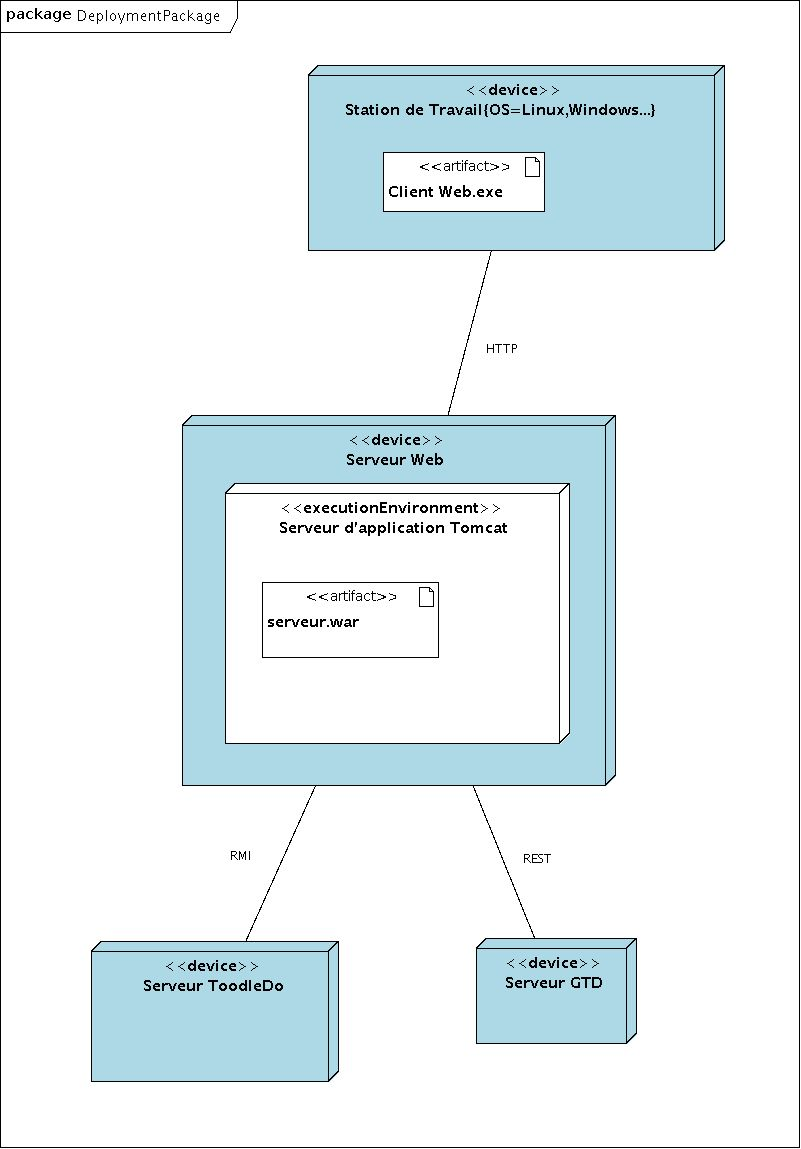
\includegraphics[scale=0.6]{livrable4/deploy.jpg}
\caption{Diagramme UML de déploiement}
\end{center}
\end{figure}



\chapter{Décisions de conceptions}

    Dans l'ensemble, nous sommes restés assez fidèle à nos idées de départ.

    \section{Communication}

    Le groupe développant le serveur GTD a fait le choix de communiquer avec les autres serveurs de manière asynchrone grâce à un système de CallBack. Le problème est que la communication entre nos composants se fait de manière synchrone, il a donc fallu mettre au point un système permettant de mettre en attente le thread effectuant la requête jusqu'à que celui-ci soit réveillé par l'appel de notre CallBack.

    \section{Synchronisation}

    Notre application faisant appel à deux serveurs GTD différents, chacun étant accessible par leur propre interface, quand l'utilisateur utilise la notre, il est nécessaire de synchroniser les données. Pour ce faire, nous nous sommes inspirés du modèle SVN, c'est à dire que lorsque par exemple l'utilisateur listera tous les projets, le serveur Web récupèrera tous les projets de chaque serveur GTD dans deux listes distinctes. Celles-ci seront remontées jusqu'à l'interface et ce sera à l'utilisateur de choisir quel projet garder parmi ceux qui diffèrent entre les 2 listes. Une fois les conflits réglés, les choix seront répercutés sur les serveurs.

    \section{Exceptions}
    
    Chaque exception levée (RMI, mauvais identifiants, Serveur GTD via le onFailure du CallBack) est remontée jusqu'à l'interface afin de prévenir l'utilisateur de tout problème éventuel.

    \section{Contraintes OCL}

    Les contraintes OCL spécifiées dans les précédents livrables sont traitées le plus tôt possible, c'est à dire au niveau de l'interface. Celle-ci guide suffisamment l'utilisateur pour éviter que ce-dernier ne saisisse par exemple une mauvaise valeur ou qu'une tâche ne dépende d'elle même.


\chapter{Conception détaillée}

    \section{Diagramme de classe}

    Comme notre architecture est assez modeste, nous n'avons pas utilisé de conteneurs de composants ou autres IOC, tout est centralisé au niveau de la classe statique WebServerManager. Celle-ci récupère les instances de chaque composant et les fournies aux autres, chacun ne peut être instancié qu'une seule fois (patron de conception "Singleton"). Cela permet une certaine indépendance entre les composants qui sont obligés de passer par la configuration (WebServerManager, cf. cours de composant), ceci afin de respecter le plus possible les concepts de la programmation par composant et de bénéficier de ses avantages (variabilités, abstraction de l'implémentation réelle, etc...). De même, l'implémentation utilise au maximum les interfaces, l'approche "mature", pour améliorer la lecture, la modularité, la maintenabilité, la variabilité, l'abstraction... du code.

\begin{figure}[H]
\begin{center}
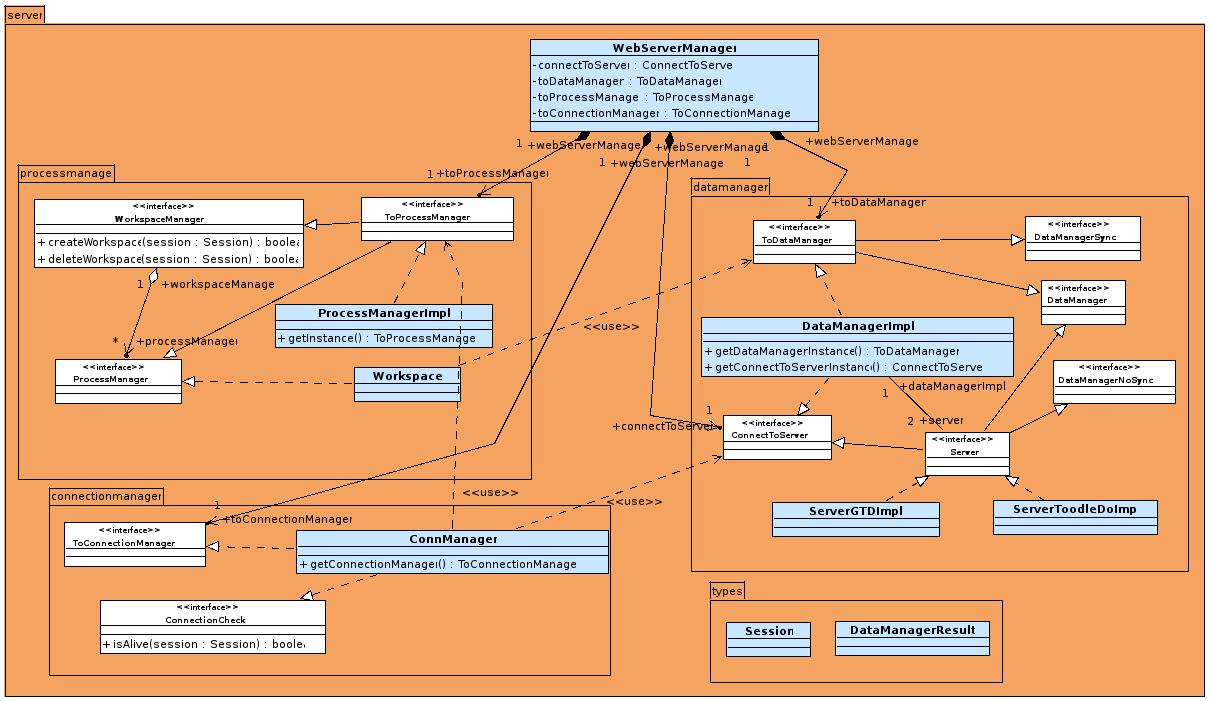
\includegraphics[scale=0.7,angle=90]{livrable4/diag_classe.jpg}
\caption{Diagramme UML de classes}
\end{center}
\end{figure}

Hormis les méthodes spécifiées dans ce diagramme de classe, toutes les autres méthodes offertes par l'interface ServeurRMI, fournie par le Serveur GTD, sont réparties ainsi : \\

\begin{itemize}
\item CRUD sur les types de bases avec synchronisation : ProcessManager, ToProcessManager, ToDataManager
\item CUD sur les types de bases : DataManager
\item R avec synchronisation : DataManagerSync
\item R sans synchronisation : DataManagerNoSync
\item connexion/déconnexion de l'utilisateur : ToConnectionManager, ConnectToServer, Server
\item CRUD sur les types de bases sans synchronisation : Server\\
\end{itemize}
\bigskip
A préciser qu'un Workspace correspond à un utilisateur. Celui-ci stocke en local les données concernant l'utilisateur afin de limiter les accès aux serveur ce qui permet indirectement d'augmenter la réactivité de l'interface.

    \section{Types de bases}
    
Les interfaces des types de bases ainsi que des implémentations de celles-ci sont fournies par l'équipe du serveur GTD. Dans notre cas, nous avons dû spécialiser ces implémentations pour pouvoir affecter nous même un identifiant à chacun de ces types nécessaire à ToodleDo, contrairement au ServeurGTD. On a pu aussi remarquer que ToodleDo ne dispose pas de tous nos concepts. Par exemple le taux d'effort pour une tâche et les idées ne sont pas présents, ces fonctionnalités ne sont donc tout simplement pas implémentées par ServeurToodleDO et ne sont pas prises en compte lors de la synchronisation. On rappelle que les types de bases sont : \\

\begin{itemize}
\item Projet
\item Tâche
\item Contexte
\item Tag
\item Idée\\
\end{itemize}

A ceux-ci, nous avons ajouté les types Session et DataManagerResult. Le premier permet de stocker les logins et mots de passes de l'utilisateur pour les deux serveurs ainsi que l'identifiant de session pour le serveur GTD et le token pour le serveur ToodleDo. Ces deux éléments sont renvoyés par leur serveur respectif lorsque l'authentification a réussi. Ils permettent d'identifier l'utilisateur auprès des serveurs et assurent ainsi la sécurité. Un objet Session est instancié quand un utilisateur se connecte et détruit quand celui-ci se déconnecte : l'identifiant et le token ne sont plus valide.\\
Le second type, DataManagerResult assure la synchronisation entre les deux serveurs. Il contient deux listes génériques, lorsque la lecture d'un type sur les deux serveurs est remontée jusqu'à DataManagerImpl, les deux listes obtenues sont stockées dans un objet DataManagerResult qui sera remonté jusqu'à l'interface.


\chapter{Scripts de génération de code}

    Du fait de notre architecture, le corps des méthodes CRUD au sein d'une classe qui implémente Serveur RMI sont quasi identiques, seul le nom des données change... voici un exemple :

\begin{verbatim}
<%for (interfaceRealization.contract.ownedOperation){%>
<%for (ownedParameter[direction == "in"]){%>
* @param <%name%>
<%}%>
<%for (ownedParameter[direction == "return"]){%>
* @return <%resolveType%>
<%}%>
*/
<%visibility%> synchronized <%ownedParameter[direction == "return"].resolveType%> <%name%>(<%ownedParameter[direction == "in"].declaration.sep(", ")%>) {

CallBackSync<String> cb = new CallBackSync<String>();
//TODO
this.wait();
if (cb.getException() != null) {
throw cb.getException();
}
return cb.getValue();
}
<%}%>
\end{verbatim}

\begin{verbatim}
<%script type="Parameter" name="resolveType"%>
<%if (upper == -1){%>List<<%type.name%>><%}else{%><%type.name%><%}%>
\end{verbatim}

On peut remarquer le système de synchronisation entre le CallBack et l'appel de méthode. Ici on passe d'une communication asynchrone à une communication synchrone : lorsque le serveur appel une des méthode du CallBack, celle-ci "notify" (réveille) l'objet appelant qui s'était mis en attente à l'instruction "wait".

La plupart des autres règles de générations de code se base sur la même structure de script, seul le corps des méthodes change. Pour gérer les importations de classes, voici le script utilisé :

\begin{verbatim}
<%script type="Class" name="gestImport"%>
<%-- superclasse --%>
<%if (superClass != null && superClass.package.name != package.name){%>
<%(superClass.package.name+"."+superClass.name).addToImport()%>
<%}%>
<%-- interfaces --%>
<%for (interfaceRealization){%>
<%(contract.package.name+"."+contract.name).addToImport()%>
<%}%>
<%-- attributs --%>
<%for (attribute){%>
<%if (type.package.name != "UMLPrimitiveTypes"){%>
<%(type.package.name+"."+type.name).addToImport()%>
<%}%><%}%>
<%-- methodes --%>
<%for (ownedOperation){%>
<%for (ownedParameter){%>
<%if (type.package.name != "UMLPrimitiveTypes"){%>
<%(type.package.name+"."+type.name).addToImport()%>
<%}%><%}%><%}%>
\end{verbatim}


\chapter{Conclusion}

    Ce projet aura été assez difficile à mener à terme. Bien qu'intéressant car celui-ci faisait appel à différentes technologies et nous permettait de mettre en pratique les divers modules enseignés ce dernier semestre, un certain manque de coordination entre les différents groupes et un manque d'expertise dans le domaine sont venus ralentir la progression.// En effet, il s'est finalement révélé que notre partie n'était en fait qu'une interface Web, aucune base de données local, aucune persistance, la partie métier de notre serveur était relativement vide. Notre développement, hormis l'interface, dépendait donc très fortement du serveur GTD central qui devait s'accorder avec les différents groupes qui n'avaient pas forcément tous la même vision des choses. Afin de rajouter de la consistance à notre serveur, nous avons inclue le serveur propriétaire ToodleDo qui possède déjà sa propre interface mais qui fournie les API nécessaires pour l'utiliser par nos propres moyens. Le problème a été que tous nos concepts n'étaient pas présent et qui fallait assurer une synchronisation entre les deux serveurs, rajoutant de la difficulté supplémentaire.// Malgré tout, cela a été une bonne expérience et nous a montré que c'est loin d'être évident de mener à bien un projet réparti en plusieurs groupes de travail tout en respectant le cahier des charges et les contraintes de temps imposées.
